\subsection{Centroid}

A  centroid of a tree is defined as a node such that when the tree is rooted at it, no other nodes have a subtree of size greater than $\frac{N}{2}$.

\begin{itemize}
  \item if $N \geq 3$ the centroid is never a leaf
  \item Every tree have a centroid.
  \item There is at most two centroids (mostly only one)
  \item All centroids are adjascent
  \item Let $s(v)$ be the sum of the distance from $v$ to every other node, essentially $\sum_{u \neq v} dist(u,v)$, then if, $c$ is the centroid, it implies that $s(c)$ is the smallest one among every other node.
\end{itemize}

\subsection{Centroid decomposition}

The centroid decomposition of a tree is another tree defined recursively as:

\begin{itemize}
  \item Its root is the centroid of the original tree.
  \item Its children are the centroid of each tree resulting from the removal of the centroid from the original tree.
\end{itemize}

Properties:

\begin{itemize}
  \item The tree formed contains all the $N$ nodes.
  \item The height of the centroid decomposition is $O()\log{N})$.
  \item Let $A$ and $B$ be two arbitrary nodes, let $C$ be the $LCA(A,B)$ in the centroid decomposition tree.
    \subitem $C$ lies on the path from $A$ to $B$ in the original tree.
    \subitem Every path in the tree can be decomposed in $A$ to $C$, and $C$ to $B$.
    \subitem As the height of the tree is $O(\log{N})$ the $LCA$ can be found in $O(\log{N})$ (just like with binary lifting)
\end{itemize}

Example:

\begin{figure}[H]
  \begin{center}
    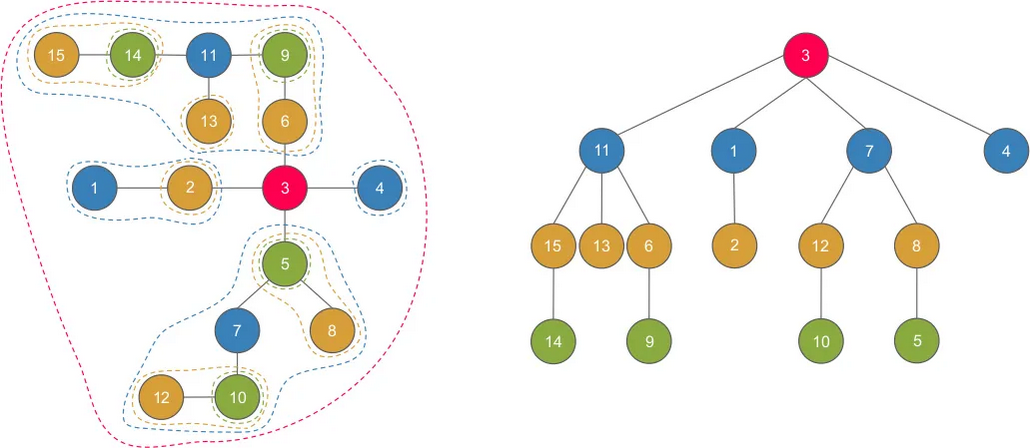
\includegraphics[width=0.45\textwidth]{media/centroidDecompositionExample.png}
  \end{center}
\end{figure}

